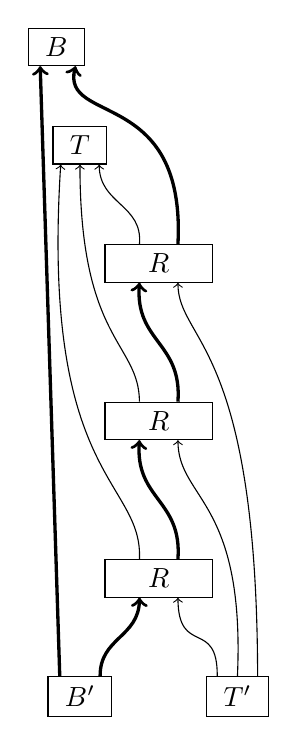
\begin{tikzpicture}[baseline=10ex]
\path (0,0) node (one) [shape=rectangle, draw] {\; \; $R$ \; \;};
\path (0,2) node (two) [shape=rectangle, draw] {\; \; $R$ \; \;};
\path (0,4) node (three) [shape=rectangle, draw] {\; \; $R$ \; \;};
\path (-1,5.5) node (T) [shape=rectangle, draw]{\;$T$\;};
\path (1,-1.5) node (T') [shape=rectangle, draw]{\;$T'$\;};
\path (-1.3,6.75) node (B) [shape=rectangle, draw]{\;$B$\;};
\path (-1,-1.5) node (B') [shape=rectangle, draw]{\;$B'$\;};

\draw [->, very thick] (one.45).. controls (.3,1) and (-.3,1) .. (two.225);
\draw [->,very thick] (two.45).. controls (.3, 3) and (-.3, 3) ..(three.225);

\draw [->] (three.135).. controls (-.2,4.75) and (-.75,4.75) .. (T.315);
\draw [->] (two.135).. controls (-.25,3)and (-1,3).. (T.270);
\draw [->] (one.135).. controls (-.2,1.25) and (-1.5,1.25).. (T.225);

\draw [<-] (one.315).. controls (.25, -1) and (.75,-.5) .. (T'.135);
\draw [<-] (two.315).. controls  (.25, 1) and (1.1,1) .. (T'.90);
\draw [<-] (three.315).. controls  (.25, 3) and(1.25,3)  .. (T'.45);

\draw [->, very thick] (three.45).. controls (.35,6.25) and (-1.25,5.75) .. (B.315);
\draw [->, very thick] (B'.135)-- (B.230);
\draw [->, very thick] (B'.45).. controls (-.75,-.75) and (-.25,-.75) ..(one.225);

\end{tikzpicture}
